%%%%%%%%%%%%%%%%%%%%%%%%%%%%%%%%%%%%%%%%%
% Make sure to set your name, legi number and url to the right git branch.
\newcommand{\hmwkAuthorName}{Julien Lamour} % Your name
\newcommand{\hmwkAuthorLegi}{13-820-907} % Your name
\newcommand{\hmwkGitBranch}{https://gitlab.vis.ethz.ch/vwegmayr/slt-coding-exercises/tree/13-820-907/1\_locally\_linear\_embedding} % Your name
%
%%%%%%%%%%%%%%%%%%%%%%%%%%%%%%%%%%%%%%%%%

%----------------------------------------------------------------------------------------
%	PACKAGES AND OTHER DOCUMENT CONFIGURATIONS
%	Skip this
%----------------------------------------------------------------------------------------

\documentclass{article}

\usepackage{fancyhdr} % Required for custom headers
\usepackage{lastpage} % Required to determine the last page for the footer
\usepackage{extramarks} % Required for headers and footers
\usepackage{graphicx} % Required to insert images
\usepackage{lipsum} % Used for inserting dummy 'Lorem ipsum' text into the template
\usepackage[font=small,labelfont=bf, skip=5pt]{caption}
\usepackage[skip=2pt]{subcaption}
\usepackage{mwe}
\usepackage{hyperref}
\usepackage{float}


% Margins
\topmargin=-0.45in
\evensidemargin=0in
\oddsidemargin=0in
\textwidth=6.5in
\textheight=9.0in
\headsep=0.25in 

\linespread{1.1} % Line spacing

% Set up the header and footer
\pagestyle{fancy}
\lhead{\hmwkAuthorName} % Top left header
\chead{\hmwkClass\ \hmwkTitle} % Top center header
\rhead{\firstxmark} % Top right header
\lfoot{\lastxmark} % Bottom left footer
\cfoot{} % Bottom center footer
\rfoot{Page\ \thepage\ of\ \pageref{LastPage}} % Bottom right footer
\renewcommand\headrulewidth{0.4pt} % Size of the header rule
\renewcommand\footrulewidth{0.4pt} % Size of the footer rule

\setlength\parindent{0pt} % Removes all indentation from paragraphs

%----------------------------------------------------------------------------------------
%	DOCUMENT STRUCTURE COMMANDS
%	Skip this
%----------------------------------------------------------------------------------------

% Header and footer for when a page split occurs within a problem environment
\newcommand{\enterProblemHeader}[1]{
\nobreak\extramarks{#1}{#1 continued on next page\ldots}\nobreak
\nobreak\extramarks{#1 (continued)}{#1 continued on next page\ldots}\nobreak
}

% Header and footer for when a page split occurs between problem environments
\newcommand{\exitProblemHeader}[1]{
\nobreak\extramarks{#1 (continued)}{#1 continued on next page\ldots}\nobreak
\nobreak\extramarks{#1}{}\nobreak
}

\setcounter{secnumdepth}{0} % Removes default section numbers
\newcounter{homeworkProblemCounter} % Creates a counter to keep track of the number of problems

\newcommand{\homeworkProblemName}{}
\newenvironment{homeworkProblem}[1][Problem \arabic{homeworkProblemCounter}]{ % Makes a new environment called homeworkProblem which takes 1 argument (custom name) but the default is "Problem #"
\stepcounter{homeworkProblemCounter} % Increase counter for number of problems
\renewcommand{\homeworkProblemName}{#1} % Assign \homeworkProblemName the name of the problem
\section{\homeworkProblemName} % Make a section in the document with the custom problem count
\enterProblemHeader{\homeworkProblemName} % Header and footer within the environment
}{
\exitProblemHeader{\homeworkProblemName} % Header and footer after the environment
}

\newcommand{\problemAnswer}[1]{ % Defines the problem answer command with the content as the only argument
\noindent\framebox[\columnwidth][c]{\begin{minipage}{0.98\columnwidth}#1\end{minipage}} % Makes the box around the problem answer and puts the content inside
}

\newcommand{\homeworkSectionName}{}
\newenvironment{homeworkSection}[1]{ % New environment for sections within homework problems, takes 1 argument - the name of the section
\renewcommand{\homeworkSectionName}{#1} % Assign \homeworkSectionName to the name of the section from the environment argument
\subsection{\homeworkSectionName} % Make a subsection with the custom name of the subsection
\enterProblemHeader{\homeworkProblemName\ [\homeworkSectionName]} % Header and footer within the environment
}{
\enterProblemHeader{\homeworkProblemName} % Header and footer after the environment
}
   
%----------------------------------------------------------------------------------------
%	NAME AND CLASS SECTION
%	Skip this
%----------------------------------------------------------------------------------------

\newcommand{\hmwkTitle}{Locally Linear Embedding} % Assignment title
\newcommand{\hmwkDueDate}{Monday,\ March\ 6th,\ 2017} % Due date
\newcommand{\hmwkClass}{SLT coding exercise\ \#1} % Course/class
\newcommand{\hmwkClassTime}{Mo 16:15} % Class/lecture time
\newcommand{\hmwkClassInstructor}{} % Teacher/lecturer

%----------------------------------------------------------------------------------------
%	TITLE PAGE
%	Skip this
%----------------------------------------------------------------------------------------

\title{
\vspace{2in}
\textmd{\small{\hmwkClass}}\\
\textmd{\textbf{\hmwkTitle}}\\
\small{https://gitlab.vis.ethz.ch/vwegmayr/slt-coding-exercises}\\
\normalsize\vspace{0.1in}\small{Due\ on\ \hmwkDueDate}
%\vspace{0.1in}\large{\textit{\hmwkClassInstructor\ \hmwkClassTime}}
\vspace{3in}
}

\author{
\hmwkAuthorName\\
\hmwkAuthorLegi
}

\date{ } % Insert date here if you want it to appear below your name

\begin{document}

\maketitle

%----------------------------------------------------------------------------------------
%	TABLE OF CONTENTS
%	Skip this
%----------------------------------------------------------------------------------------

%\setcounter{tocdepth}{1} % Uncomment this line if you don't want subsections listed in the ToC

\newpage
\tableofcontents
\newpage

%----------------------------------------------------------------------------------------
%	SECTIONS
%	Now you are in the right hood
%----------------------------------------------------------------------------------------

\begin{homeworkProblem}[The Model]
The model section is intended to allow you to recapitulate the essential ingredients used in \hmwkTitle. Write down the \textit{necessary} equations to specify \hmwkTitle\ and and shortly explain the variables that are involved. This section should only introduce the equations, their solution should be outlined in the implementation section.\newline
Hard limit: One page
\vspace{10pt}

\problemAnswer{ % Answer
Cost function for reconstruction errors:
\begin{equation}
    \mathcal{E}(W)=\sum_i{\Bigl|\vec{X_i} - \sum_j{W_{ij}\vec{X_j}}\Bigr|^2}
\end{equation}
\hspace{3pt} where $\vec{X_i}$ is the point to be reconstructed from a weighted combination ($W_{ij} $for$ j=1...n$) of its neighbors $\vec{X_j}$. $\sum_{ij}W_{ij}=1$ and $W_{ij}=0$ if $\vec{X_i}$ and $\vec{X_j}$ are not neighbors.\\

Cost function for low dimensional coordinates:
\begin{equation}
    \Phi(Y) = \sum_i{\Bigl|\vec{Y_i}-\sum_j{W_{ij}\vec{Y_j}}\Bigr|^2}
\end{equation}
\hspace{3pt} where $W_{ij}$ are the exact same weights are described earlier and $\vec{Y_i}$ is the lower dimensional vector corresponding to $\vec{X_i}$ in the initial dimension.
}
\end{homeworkProblem}
\clearpage

%----------------------------------------------------------------------------------------
\begin{homeworkProblem}[The Questions]
\begin{homeworkSection}{(a) Get the data}
I used a subset of the training set of size $N=5000$ for the exercise in order to get acceptable runtime. I made a few tests with the whole dataset ($N=60000$) but the results were similar.
\end{homeworkSection}
\begin{homeworkSection}{(b) Locally linear embedding}
We can observe that both in 2D and 3D it is possible to see clusters in the data. Since the influence on the number of neighbors is studied in a later question, these plots were done using the 10 nearest neighbors for each points.
\begin{figure}[H]
    \centering
    \begin{subfigure}[b]{0.46\textwidth}
        \centering
        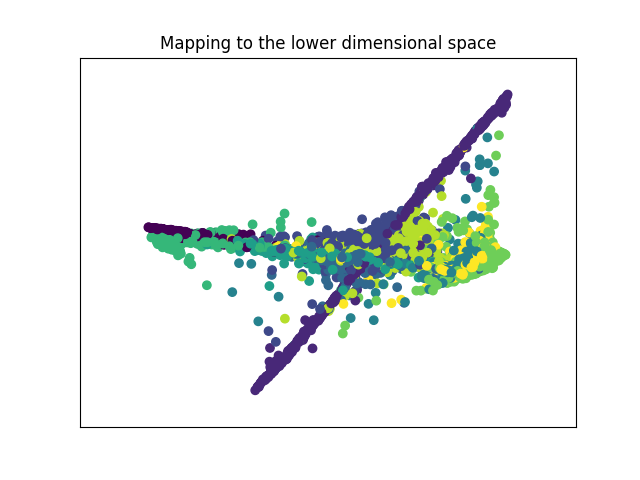
\includegraphics[width=\textwidth]{images/Y210.png}
        \caption[Network2]%
        {{\small 2D}}    
        \label{fig:y2-10}
    \end{subfigure}
    \hfill
    \begin{subfigure}[b]{0.48\textwidth}  
        \centering 
        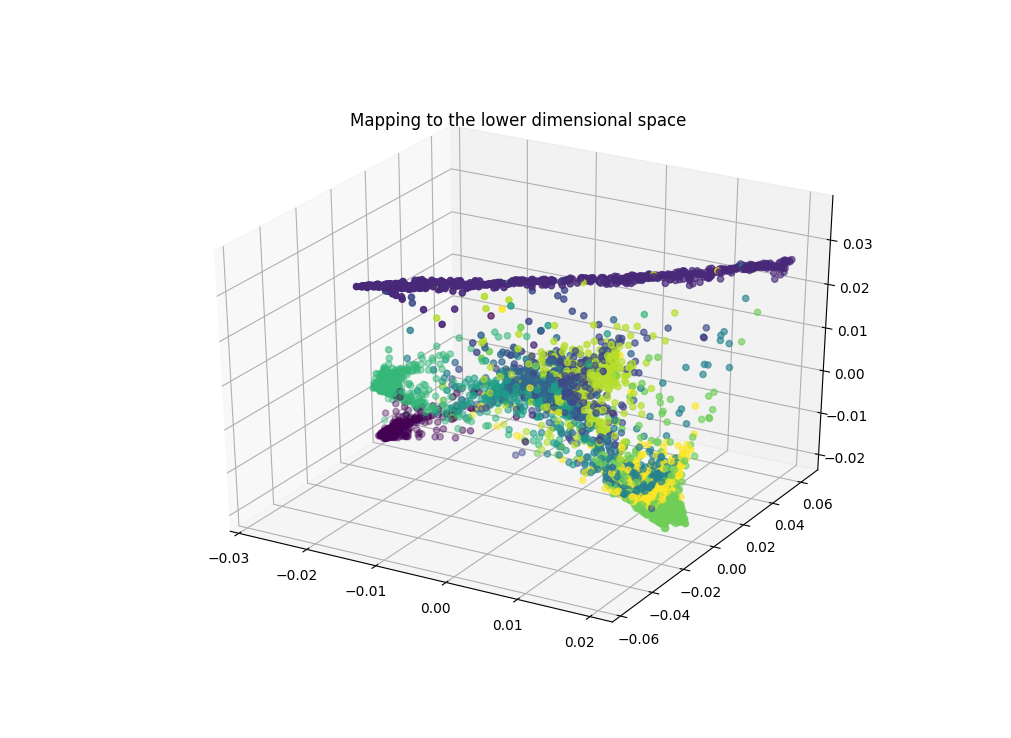
\includegraphics[width=\textwidth]{images/Y310-1.png}
        \caption[]%
        {{\small 3D}}    
        \label{fig:y3-10-1}
    \end{subfigure}
    \caption[ Visualizations for 2D and 3D embedding spaces.]
    {\small Visualizations for 2D (a) and 3D (b-d) embedding spaces.} 
    \label{fig:visualizations}
\end{figure}
\end{homeworkSection}
\begin{homeworkSection}{(c) Cluster structure}
As we can observe on the following plots, the M matrix has values very close to zero everywhere but in the diagonal and singular values are concentrated close to 0. Since the optimal embedding is found by computing the botton $d+1$ eigenvectors of the matrix $M$, one could start from 1D and stop adding eigenvectors (i.e. increasing the embedding dimension) until there is no significant gain in the reconstruction error.
\begin{figure}[H]
    \centering
    \begin{subfigure}[b]{0.4\textwidth}
        \centering
        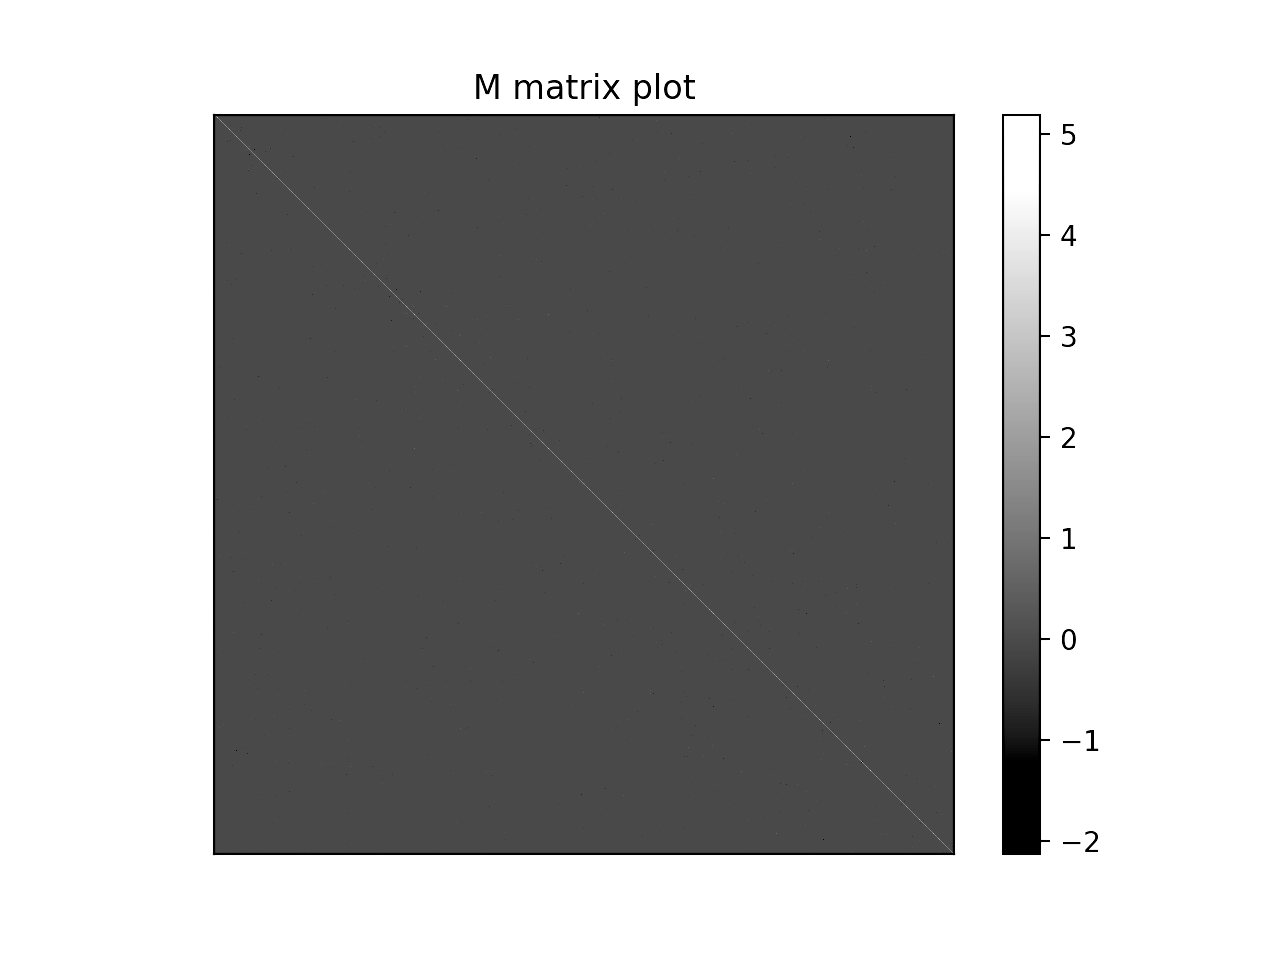
\includegraphics[width=\textwidth]{images/M_2-3_10.png}
        \caption[]%
        {{\small M Matrix plot}}    
        \label{fig:M}
    \end{subfigure}
    \hfill
    \begin{subfigure}[b]{0.4\textwidth}  
        \centering 
        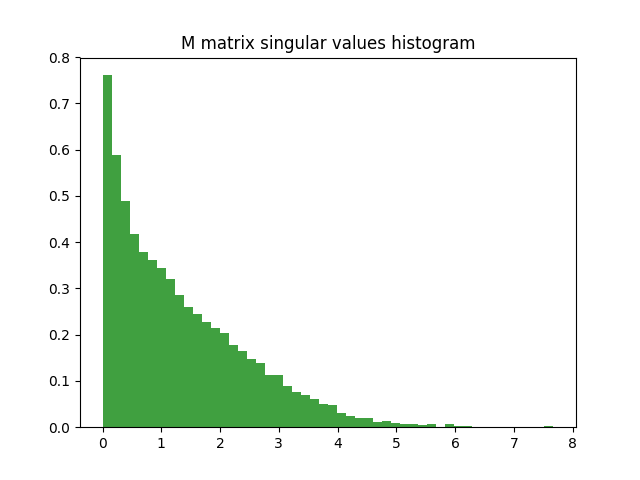
\includegraphics[width=\textwidth]{images/sing_2-3_10_hist.png}
        \caption[]%
        {{\small Histogram for M matrix singular values}}    
        \label{fig:sing}
    \end{subfigure}
    \caption[ Cluster structure of the data]
    {\small Cluster structure of the data.} 
    \label{fig:structure}
\end{figure}
\end{homeworkSection}
\begin{homeworkSection}{(d) Nearest Neighbors}
\begin{figure}[H]
    \centering
    \begin{subfigure}[b]{0.32\textwidth}
        \centering
        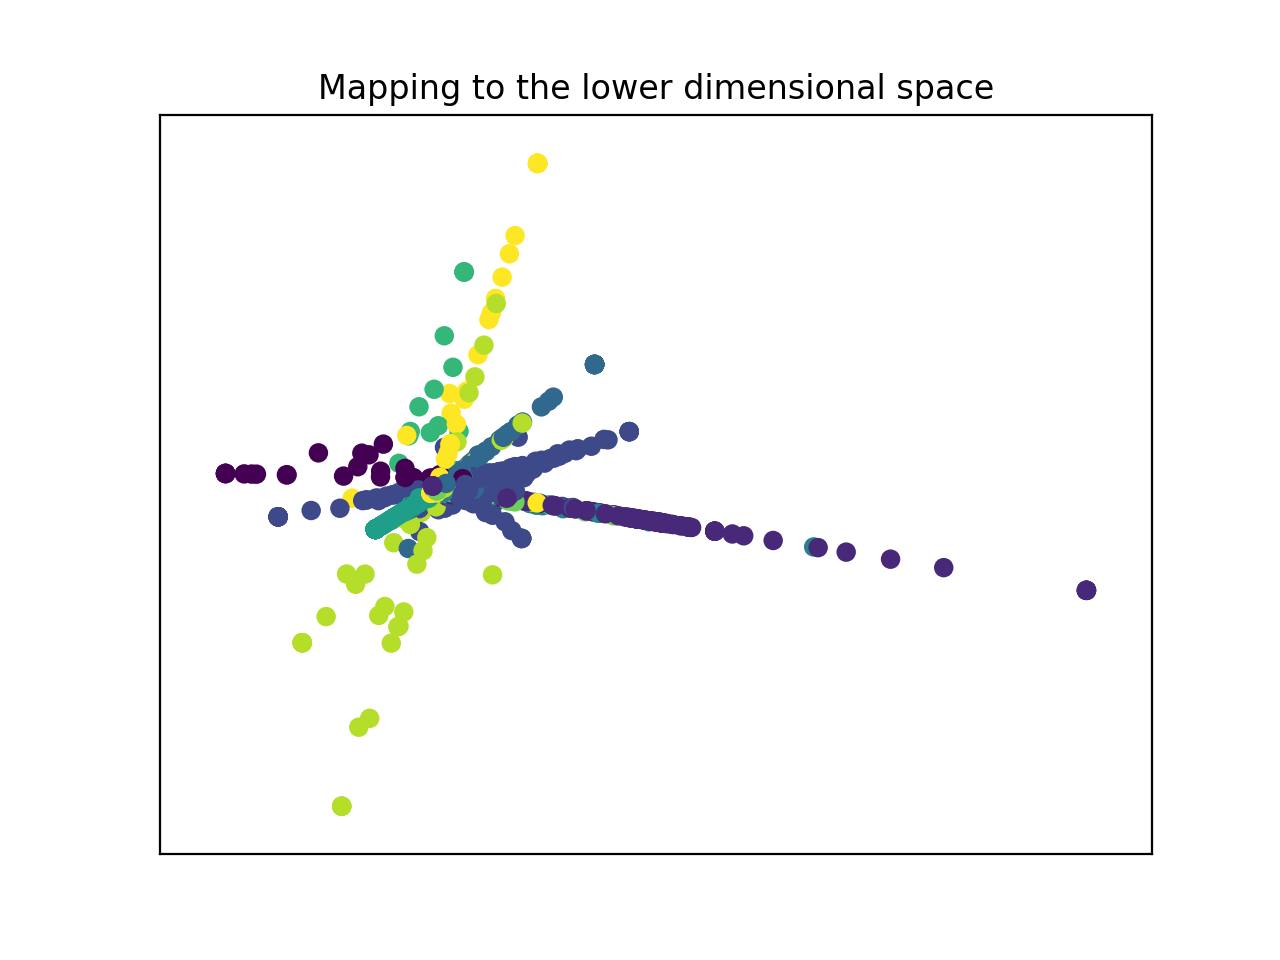
\includegraphics[width=\textwidth]{images/k3_euc.png}
        \caption[]%
        {{\small 3 neighbors}}    
        \label{fig:3neighbors}
    \end{subfigure}
    \hfill
    \begin{subfigure}[b]{0.32\textwidth}  
        \centering 
        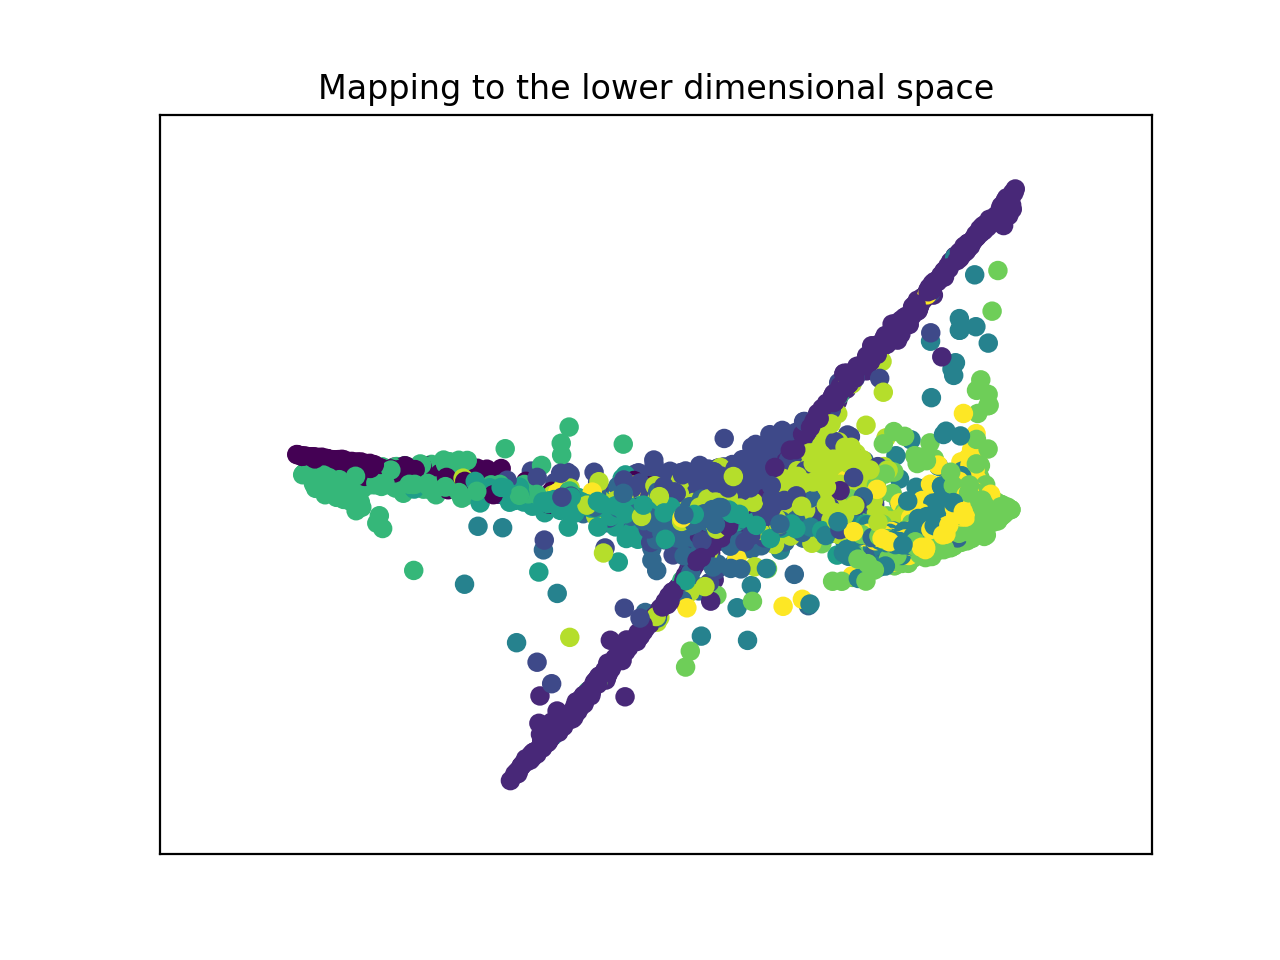
\includegraphics[width=\textwidth]{images/k10_euc.png}
        \caption[]%
        {{\small 10 neighbors}}    
        \label{fig:10neighbors}
    \end{subfigure}
        \begin{subfigure}[b]{0.32\textwidth}
        \centering
        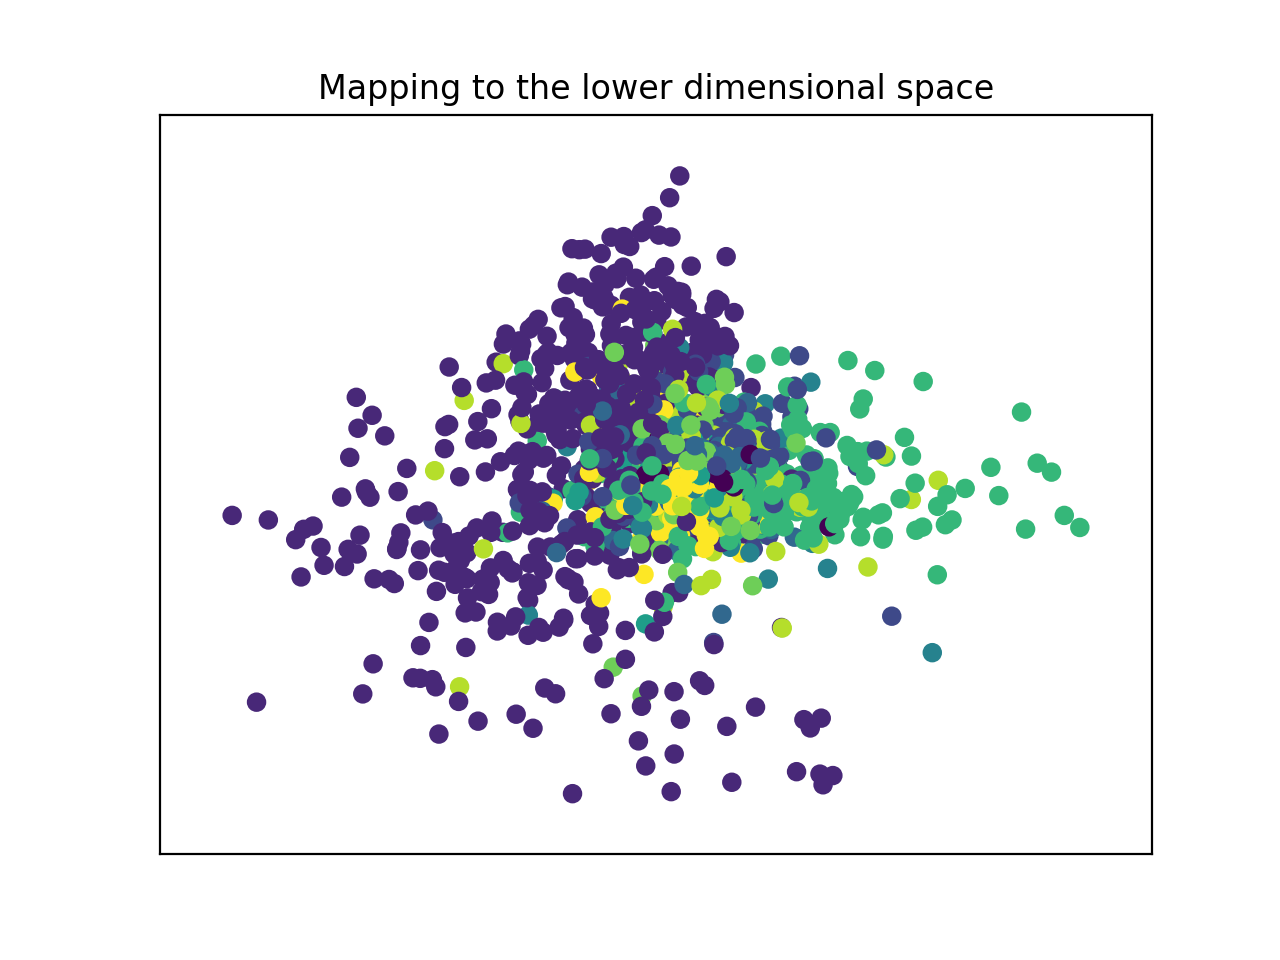
\includegraphics[width=\textwidth]{images/k35_euc.png}
        \caption[]%
        {{\small 35 neighbors}}    
        \label{fig:35neighbors}
    \end{subfigure}
    \hfill
    \caption[]
    {\small Influence of the number of neighbors $k$ (using Euclidean norm).}
    \label{fig:neighbors}
\end{figure}
\begin{figure}[H]
    \centering
    \begin{subfigure}[b]{0.32\textwidth}
        \centering
        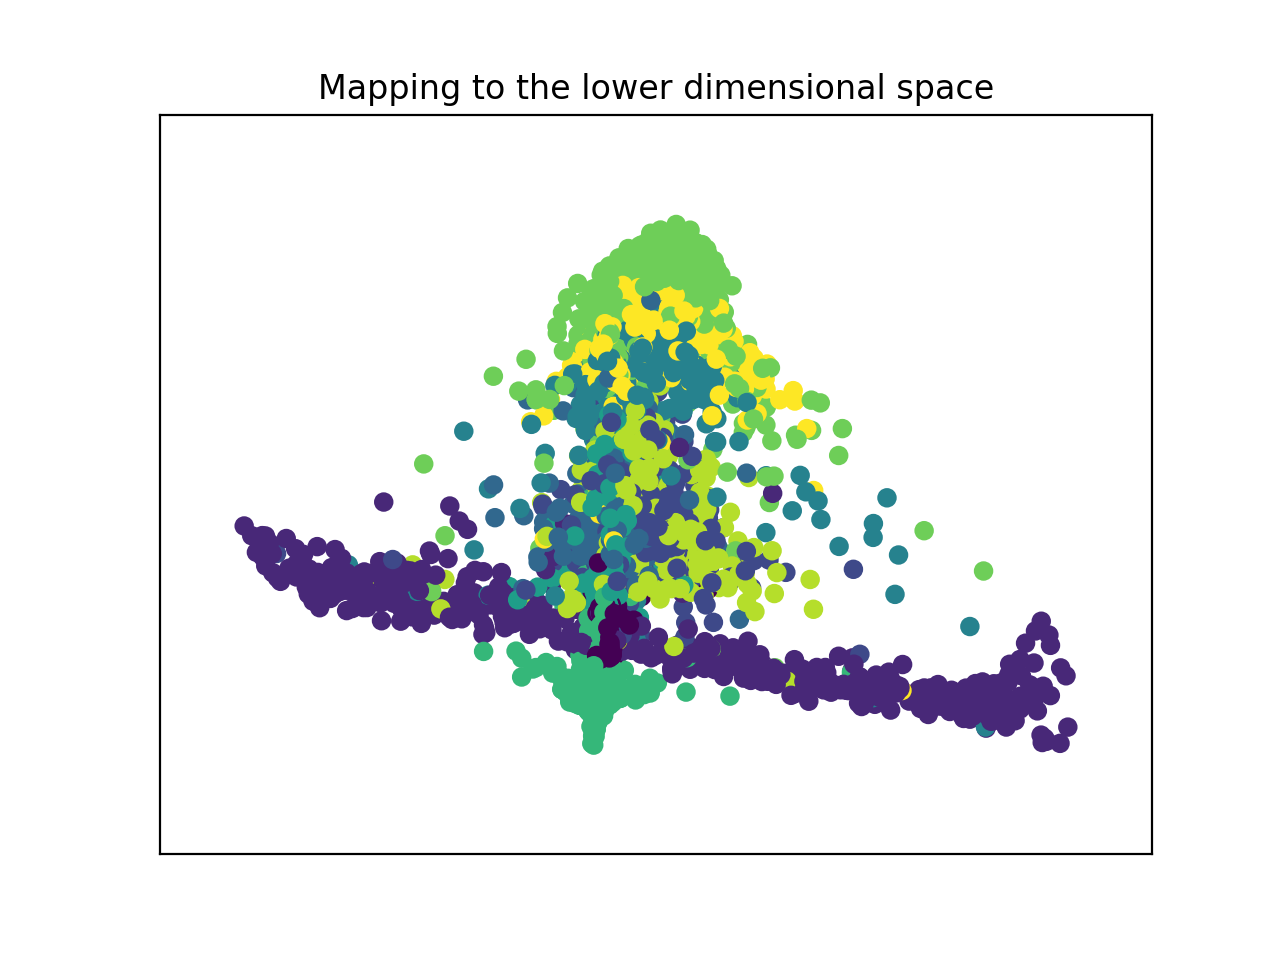
\includegraphics[width=\textwidth]{images/15_n1.png}
        \caption[]%
        {{\small L-1 norm}}    
        \label{fig:l1}
    \end{subfigure}
    \hfill
    \begin{subfigure}[b]{0.32\textwidth}  
        \centering 
        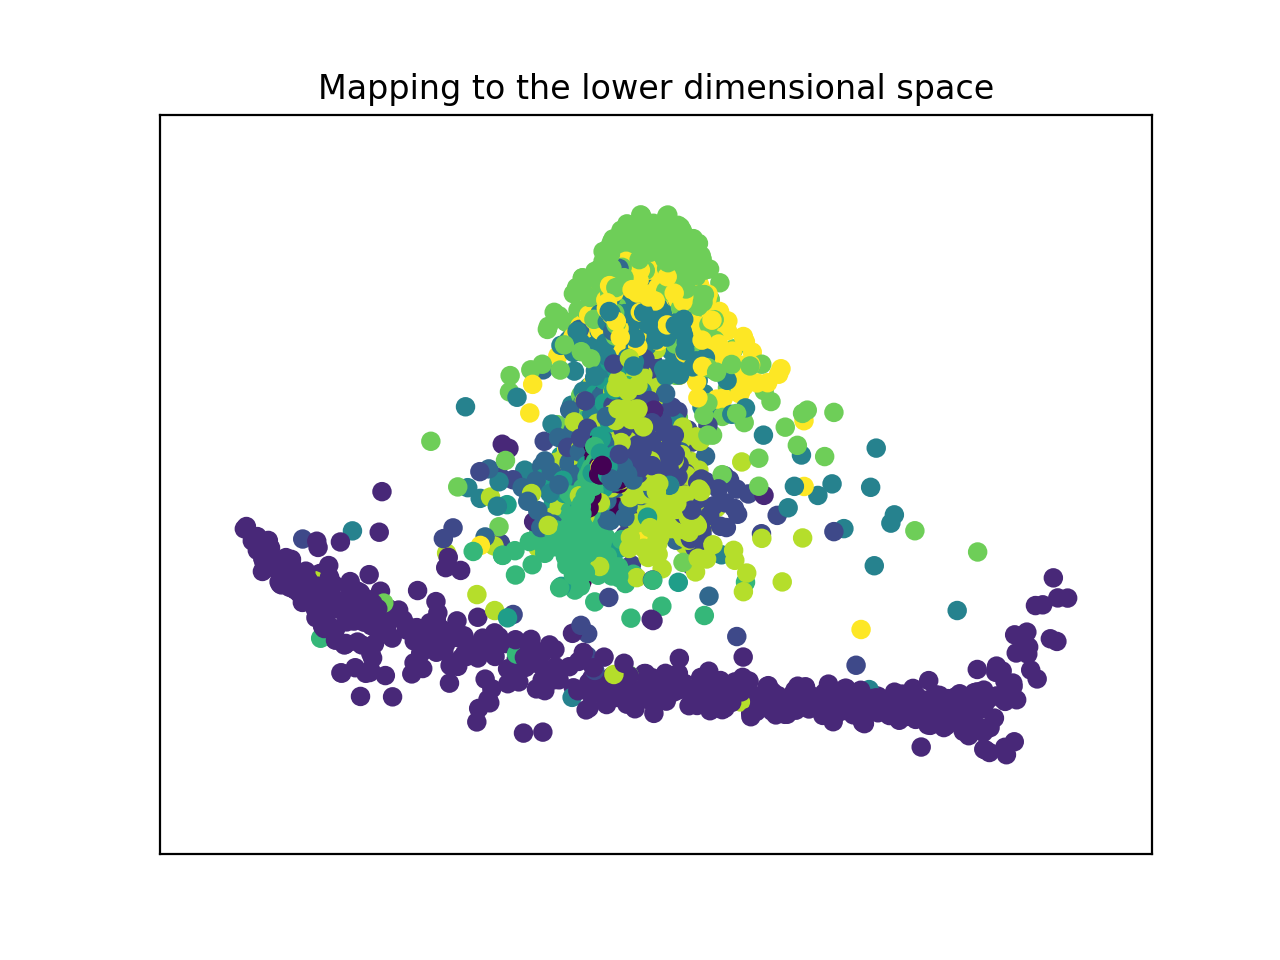
\includegraphics[width=\textwidth]{images/15_n2.png}
        \caption[]%
        {{\small L-2 norm}}    
        \label{fig:l2}
    \end{subfigure}
        \begin{subfigure}[b]{0.32\textwidth}
        \centering
        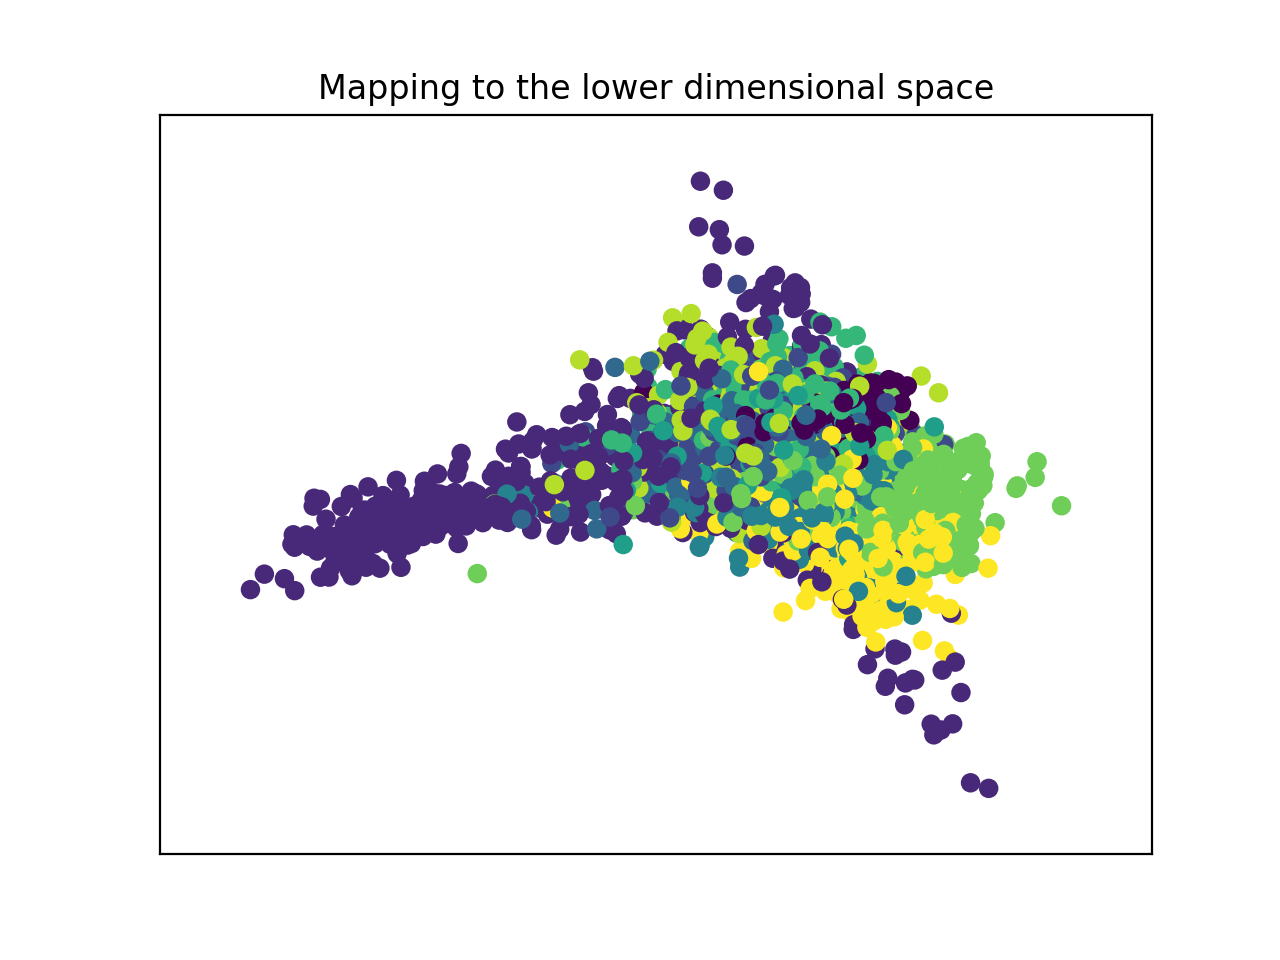
\includegraphics[width=\textwidth]{images/15_ninf.png}
        \caption[]%
        {{\small L-$\infty$ norm = $max(abs(x))$}}    
        \label{fig:linf}
    \end{subfigure}
    \hfill
    \caption[]
    {\small Usage of different norms with fixed number of neighbors (15).}
    \label{fig:norms}
\end{figure}
As we can observe of the above plots, the number of neighbors $k$ strongly influences the mapping in the lower dimensional space. Literature shows that it is usually common to pick $k$ by cross validation. Different norms also leads to different results, which can be trivially explained by the facts that different neighbors are going to be picked, but it has less influence than the number of neighbors.
\end{homeworkSection}
\begin{homeworkSection}{(e) Linear manifold interpolation}


Assume you pick some point in the embedding space. How can you map it back to the original (high dimensional) space? Investigate how well this works for points within and outside the manifold (does it depend on the dimensionality of the embedding space?) Try things like linearly interpolating between two embedding vectors and plot the sequence of images along that line. What happens if you do that in the original space?
\end{homeworkSection}
\end{homeworkProblem}
\clearpage

%----------------------------------------------------------------------------------------
\begin{homeworkProblem}[The Implementation]
In the implementation section you give a concise insight to the practical aspects of this coding exercise. It mainly mentions the optimization methods used to solve the model equations. Did you encounter numerical or efficiency problems? If yes, how did you solve them?
Provide the link to your git branch of this coding exercise.\newline
Hard limit: One page

\vspace{10pt}
\problemAnswer{ % Answer
I used Numpy for system solving as well as for eigenvalues computation, which is already optimized and therefore didn't lead to numerical neither efficiency problems. I used Matplotlib for plotting. I could have used a library for faster nearest-neighbors computation but found it more interesting to have it written by myself since it is fairly simple and makes the code more readable.\\\\
Git branch: \url{\hmwkGitBranch}
}
\end{homeworkProblem}
\clearpage

%----------------------------------------------------------------------------------------
\begin{homeworkProblem}[Your Page]
Your page gives you space to include ideas, observations and results which do not fall into the categories provided by us. You can also use it as an appendix to include things which did not have space in the other sections.\newline
No page limit.

\vspace{10pt}
\problemAnswer{ % Answer
Your Answer

\hmwkGitBranch % defined in line 5
}
\end{homeworkProblem}
\clearpage

\end{document}

